\section{Group Recommender System}
\begin{frame}
     \begin{center}
     	\huge Previous Semester
     \end{center}
\end{frame}

\begin{frame}
\frametitle{Previous Semester}
\textit{How can recommendations be made to a group of people by reflecting a groups decision making process, ensuring a high level of satisfaction in the group?}
\end{frame}

\begin{frame}
\frametitle{Previous Semester}
Working with the assumption that Borda Count could be improved

\begin{itemize}
\item Borda Transferable Count - Mix of Borda Count and Single Transferable Vote
\item Borda Escalating Count - Having a multiplication factor depending on the item rank
\item Borda Weighted Count - Gets assigned additional points based on the amount if lists an item occurs on
\end{itemize}
\end{frame}

\begin{frame}
\frametitle{Thesis Questions}
\begin{itemize}
\item How does Borda Count perform compared to state-for-the-art rank aggregation methods?
\item How does Borda Count perform on a dataset for group recommendation?
\item How does rearranging top-k lists influence the groups satisfaction?
\end{itemize}
\end{frame}

\begin{frame}
     \begin{center}
     	\huge This Semester
     \end{center}
\end{frame}

\begin{frame}
\frametitle{Group Recommendation System}
\begin{figure}
\centering
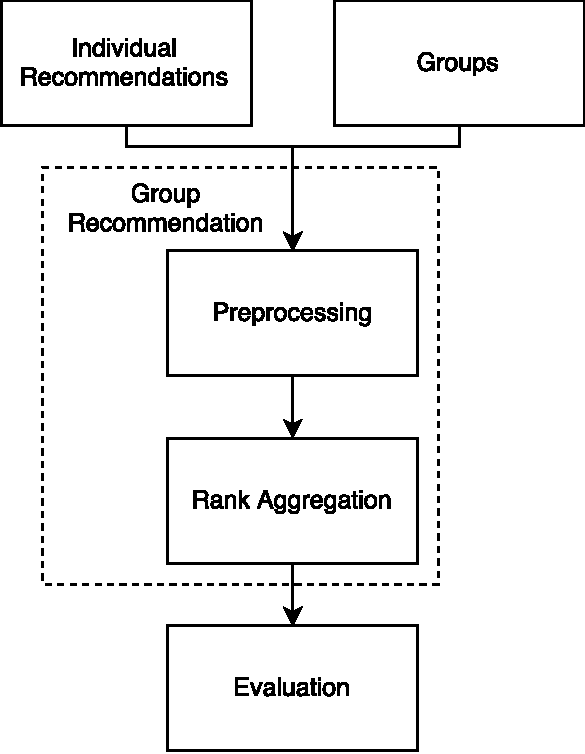
\includegraphics[scale=.5]{graphics/composition}
\end{figure}
\end{frame}

\begin{frame}
\frametitle{Alternative Aggregation Methods}
	\begin{columns}
		\begin{column}{0.5\textwidth}
		Voting systems
\begin{itemize}
\item Borda Count
\end{itemize}
Graph based methods
\begin{itemize}
\item Markov Chain 
\item Spearman's Footrule
\end{itemize}
Others
\begin{itemize}
\item Average
\end{itemize}
		\end{column}
		\begin{column}{0.5\textwidth}
		\begin{figure}
		\centering
		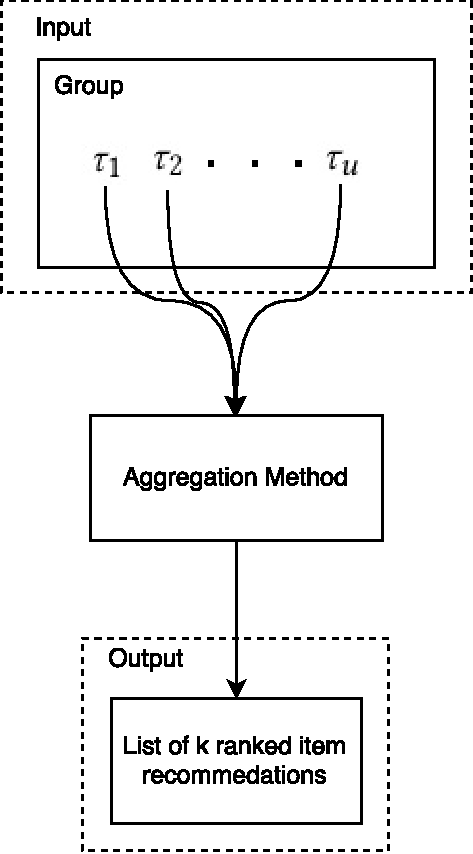
\includegraphics[scale=.4]{graphics/setuptransposed}
		\end{figure}
		\end{column}
\end{columns}
\end{frame}

%\begin{frame}
%\frametitle{Aggregation Methods}
%
%\end{frame}